As people search online to plan trips or shop for new products, they encounter many entities (e.g., museums, restaurants, camera models) and collect evidence to make decisions (e.g., travel blogs, top ten lists). Current browsers treats entities and evidence from each webpage independently of other pages, making it difficult for users to keep track of what they are interested in and why. We introduce Fusion, a novel browser addon that weaves pages together through common entities in a interface integrated into users' natural browsing experience. When users open a webpage, Fusion ``infuses'' it with information extracted from other webpages and knowledge bases relevant to entities on the current page. When users save notes about an entity, their notes are ``diffused'' across other pages where the same entity was mentioned. In evaluation, we found users valued both infusion and diffusion based features, and identified implications for the design of future browser interfaces.


\section{Introduction}

Whether planning a trip to a new city, figuring out which camera to purchase, or researching the different treatments for a medical issue, people spend a significant amount of time gathering evidence across multiple webpages to make decisions. Unlike simple searches that may require finding only a single trusted source, such as the address of a restaurant or checking the weather, complex exploratory search tasks often involve performing multiple searches and require significant amounts of learning, cross-referencing, and synthesis across multiple webpages. Consider for example planning a trip: there may be hundreds of possible restaurants to dine at, attractions to see, and places to stay, each with corresponding evidence about its suitability for an individual's goals. Evidence about each of these entities is often spread out across many different pages, including Yelp or TripAdvisor reviews, travel blogs, discussion forums, top ten lists, and travel guides. Furthermore, each piece of evidence on its own may be susceptible to its creators' biases, context, and opinion, requiring users to synthesize across many pieces of evidence and entities in order to build a reliable landscape of the decision space. Research estimates of the amount of time spent gathering and synthesizing evidence for such complex search tasks to be up to 33\% of the time spent online, which amounts to a total of more than 24 billion hours per year in the US alone (as of 2009) \cite{mar2006exp,kellar2007field,rose2004understanding,forrester}.

Significant research has gone into supporting various aspects of the above activities. One major thread of research has been around knowledge graphs composed of entities and how they relate to each other \cite{dbpedia}. These entities can then be surfaced to the user, typically by search engines alongside search results. In these systems, entities are presented as a card or a list of names, often with corresponding images \cite{bota}. While such approaches focus on and can be effective in helping users discover what entities are related to a particular information need (e.g., \cite{miliaraki2015selena}), simply knowing about the existence of an entity may only be the beginning of users' information needs. Without an understanding of context -- which web sources mention an entity, how it is mentioned across those sources, what aspects of those mentions are relevant to users' goals, and how it compares to alternative entities -- users might not know which entities are trustworthy and relevant to their goals.


To understand the prevalence of this problem, we conducted a pilot survey with 103 participants from Amazon Mechanical Turk (age between 20 and 63, M=36, SD=12, 60\% male and 40\% female, mostly from the US), focusing on their experiences when conducting complex exploratory searches. Our results reaffirm that when conducting exploratory searches, people read from multiple information sources to make sure they do not miss something important (84\%), look for more information about a topic from other webpages in the same search result (84\%), verify previously seen but uncertain information using multiple sources (88\%), and get a sense of what's popular or important in the search results (76\%). At the same time, many also found that conducting complex searches can be stressful (60\%), and that they often end up with more browser tabs than they can manage efficiently (67\%).

Another thread of addressing the problem has been tools for helping users gather and save snippets of evidence across many pages. Such tools have become popular and widespread in recent years, including Evernote with over 200 million users and Pocket with over 2 billion items saved. Researchers have also explored ways to support saving information on the web, reducing the costs and extending the capabilities of such tools, for example support saving structured data \cite{thresher,bier2006entity}. However, such systems have typically focused on creating separate environments to save and organize the collected snippets.  Accessing a separate system for context every time users encounter an item can incur significant challenges, with the costs of re-finding items in that system becoming prohibitive \cite{notetoself}.

In this paper we explore an alternative approach that scaffolds users' natural browsing experience to help them gather and synthesize evidence about entities across multiple webpages. The key insight we build on is that while users aim to collect evidence for entities across multiple sources, their browsers currently treat each of the instances of those entities as independent. If we instead understood that the same entity was being mentioned on multiple different pages, we could develop novel systems that can better support users in understanding the contexts that entity was mentioned in and how those contexts relate to their personalized needs and goals. Here we introduce one such system, Fusion, which instantiates this approach in a prototype browser addon. Fusion analyzes and identifies entities mentioned in individual pages, helping the user gradually build up a workspace of options and evidence that persists across webpages throughout the task. Using an entity-centric approach has the potential to not only reduce the costs of keeping track of options and gathering evidence, but also enables new end-user interface approaches, such as proactively showing a user how many sources mention an entity and the contexts in which it is mentioned, or propagating a users' notes and annotations across all pages an entity is cited.

The core contribution of this paper is an entity-centric approach for supporting sensemaking across webpages in the browser when conducting complex exploratory search tasks, which includes the following:

\begin{figure}
    \centering
    \frame{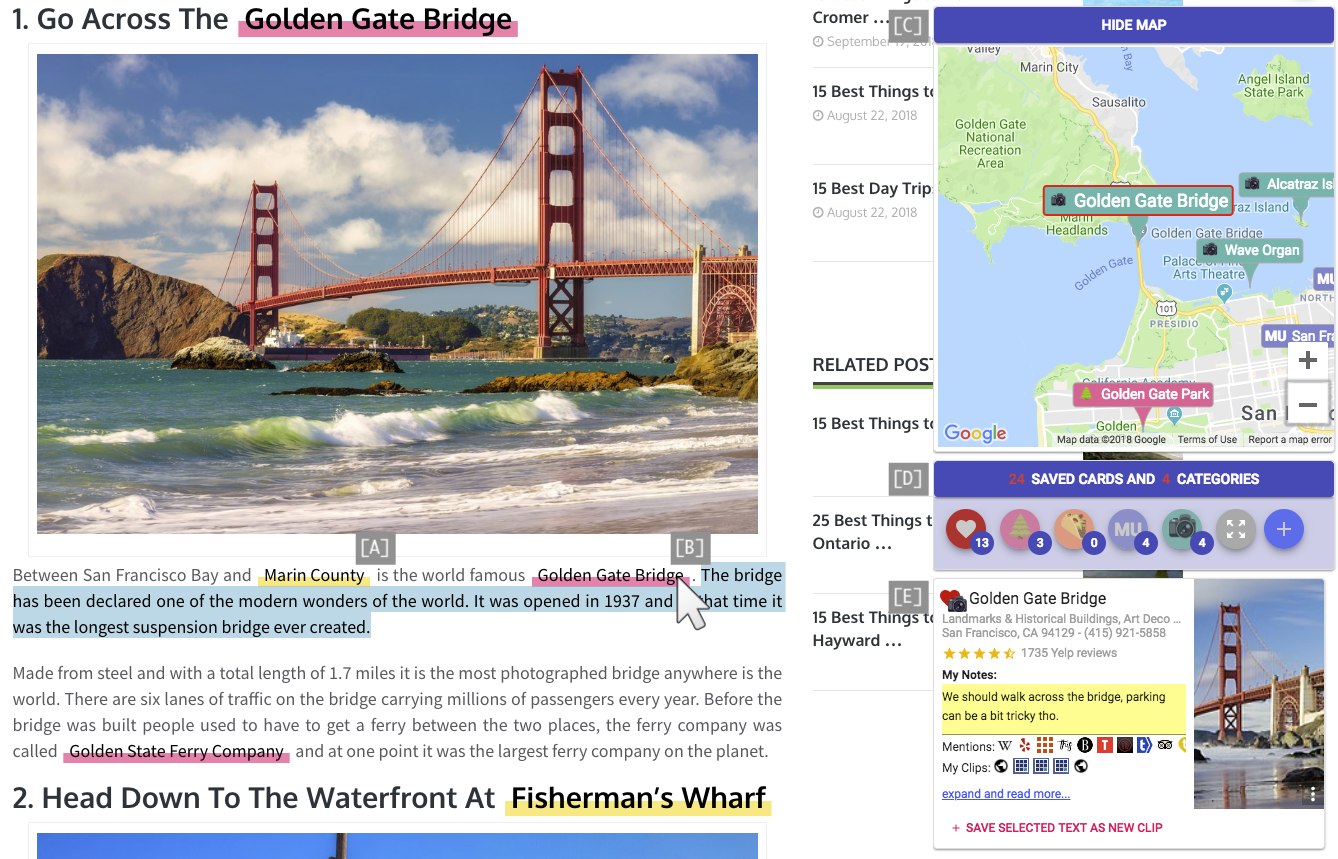
\includegraphics[width=1\textwidth]{Chapters/Fusion/main2.png}}
    \caption{An overview of the Fusion browser addon. Fusion identifies and highlights entity mentions on webpages (A,B), indicating additional information is available. Highlights in red (B) indicates users had previously interact with the entity. Hovering an entity mention (B) brings out its corresponding Entity Card (E) as an overlay, with relevant information ``infused'' from other pages and external knowledge sources as \emph{mentions}. Users can also save notes or selected sentences to a card as \emph{clips}. Saved clips are then automatically ``diffused'' to other webpages that contained the same entity. Users can also create categories (D) and drag the card under them. Finally, the Map view (C) shows its location in the context of previously saved entities.}
    \label{fig:main}
\end{figure}


\begin{itemize}
\item Fusion, a browser addon that enables the browser to better understand the content of webpages by identifying entities using existing natural language processing algorithms and external knowledge sources (e.g., Wikipedia and Yelp).
\item Support for reading and gathering information in unfamiliar domains during exploratory search tasks by lowering the cost of cross-referencing different entities across webpages and searches
\item A context-aware workspace where users can easily gather evidence from multiple webpages for a collection of entities which propagates to other pages that mentions the same entities. Allowing the system to surface relevant  information saved previously as users browse different pages.
\end{itemize}

\section{Related Work}

\subsection{Search Engines and Exploratory Search}

Research on interfaces that support exploratory search tasks have focused on providing overviews of information within search results or managing multiple searches, so searchers can better orient themselves in an unfamiliar information space \cite{hearst2009search,marchionini2000agileviews,patterson2001predicting,tretter2013searchpanel,morris2008searchbar}. Recent research has also explore ways to support managing multiple search sessions and project using novel browser interfaces \cite{hahn2018bento}. On the other end of the process, recent researchers have also explored ways to support learning by enriching and personalizing  search results when users conduct exploratory searches \cite{syed2017optimizing}. Alternatively, studies have also shown the benefits for surfacing related entities from external knowledge bases on the search results page for quick reference \cite{bota,miliaraki2015selena}, forming subsequent query terms\cite{klouche2015designing}, or collaboration \cite{andolina2018querytogether,klouche2018hyperlinks}. However, ranking algorithms and interactive search result interfaces provide little support once users opened webpages from the results to read and collect information from. At this stage of the process, not only are the individual webpages disconnected from the search results once opened, these webpages typically contain overlapping information around the same topics but are also treated as independent of each other, requiring users to manually identify common themes in different sources and collect evidence for synthesis.

While Fusion also identifies relevant entities and presents users with information from external knowledge bases, it uses this information to support lightweight cross-reference between webpages  in their search results while reading individual webpages without opening multiple tabs and switching between them, and also to support lightweight cross-referencing of users' own notes saved from different pages.

\subsection{Saving and Organizing Information}

When reading the individual pages, users in exploratory search tasks often need to take notes or save information from different webpages. Due to its ubiquity and importance, researchers have also been developing systems that can better support saving and organizing information to facilitate learning and exploratory search tasks \cite{schilit1998beyond, tashman2011liquidtext,hinckley2012informal,kittur2013costs,notetoself,chang2016supporting}. 
However, researchers have also identified common issues users are faced with while organizing collected information. Karger et al. pointed to the fact that most information management systems failed to provide effective structure for its users due to the long-tail distribution of information types that people have \cite{whatwentwrong}. Further, Kittur et al. found that in early stages of exploration, often searchers themselves do not have enough context to come up with effective structures \cite{kittur2013costs}. These studies revealed systems that force schematization too early in the exploration process stages to can be detrimental to their users. In a study closely related to our work, the NoteToSelf system added a sidebar to the browser for saving free-form notes that persist as users browse different webpages \cite{notetoself}. However, they found that while participants created many notes during browsing, they rarely revisited these notes nor deleted unused notes. This suggests that even though allowing users to externalize their arbitrary structures can be beneficial, but the high cost of recalling and re-finding previously saved information can still be prohibitive.

In our work, we address the information reuse problem using an entity-centric approach. As users opened a new webpage, Fusion analyzes the content and resurfaces previously saved notes that were associated with entities also on the current webpage in real-time. Similar to \cite{notetoself}, we also used a lightweight interface that is embedded into users' natural reading process, and allowed them to either type notes or extract content from different webpages. In our study, users expressed how this allowed them to quickly refer back to what they have learned in the past, and also reduced the cost of removing previously saved information that were no longer relevant. 

\subsection{Identifying Entity Mentions in Web Content}

There has been significant previous work in identifying entities from unstructured or semi-structured webpages. Approaches include wrapper induction techniques based on user interaction \cite{thresher}, which typically rely on multiple pages with a common structure or data format \cite{pasupat2014zero}; natural language patterns (e.g., \cite{hearst1992automatic} and \cite{fader2011identifying}) which use seed examples; or exploit regularities in semi-structured data \cite{thresher}. Our work builds on these advances in entity extraction by using a state-of-the-art entity linking algorithms for the DBpedia knowledge base \cite{spotlight,dbpedia}, and a custom algorithm for disambiguating entities across DBpedia and Yelp. However, as pointed out by Klouche \cite{klouche2018hyperlinks}, while extant approaches to entity extraction have mainly focused on search engine or question answering outcomes, there is a largely unexplored design space around using entities to drive novel end-user interactions. Our work explores one such paradigm in which entities are used to scaffold the gathering and synthesis in a user's online sensemaking process. Similar to \cite{thresher}, we also allowed users to manually extract entities from webpages, but mainly as a way to recover from errors made by the automatic entity linking algorithm \cite{spotlight}.

\section{System Design}
We introduce Fusion, a novel browser addon that uses an entity-centric approach to facilitate sensemaking across webpages in exploratory search tasks. Figure \ref{fig:main} shows an overview of how an exploratory searcher planning a trip might use Fusion. Unlike previous approaches for supporting sensemaking in exploratory search tasks, such as re-ranking or enriching the search result lists or using external note management interfaces \cite{syed2017optimizing,miliaraki2015selena}, we focused on providing \emph{in situ} support for sensemaking while reading and capturing information.  Fusion provides users a lightweight overlay interface embedded and synced across webpages in exploratory tasks, allowing users to make quick and lightweight cross-referencing without switching between tabs, windows, or applications. The two core components of Fusion augment content in two ways, which we introduce as ``\emph{infusion}'' and ``\emph{diffusion}''. First, when users open a webpage from their search results, the system ``infuses'' the webpage with relevant snippets about mentioned entities from other webpages in their search results and external knowledge sources to help users cross-reference and evaluate newly encountered options. Second, when users save notes or extract content from a webpage, the system ``diffuses'' them to related entities in other webpages in the same task, allowing them to easily access previously saved information without having to switch to and search through a separate interface \cite{notetoself}. To drive these operations and connect the different webpages, we use the DBpedia Spotlight algorithm \cite{spotlight} to automatically identify common entities mentioned in the different webpages. In our implementation, we use Yelp and DBpedia as our entity repositories and focus on travel planning tasks, but other knowledge bases can also be used or added to support other types of projects. For example, using the Microsoft Academic Graph\footnote{https://www.microsoft.com/en-us/research/project/microsoft-academic-graph/} and the Gene Ontology \cite{gene} as knowledge bases to support literature review projects in biology. In the next subsections, we will first describe in detail how Fusion identifies entities in web content, and then describe both the infusion- and diffusion-based features.

\subsection{System Architecture}
Users can create projects for different search tasks in Fusion and add searches or webpages to the project. When a search is added to a Fusion project, Fusion parses the HTML of the search results page to obtain a list of linked webpages for further processing. Alternatively, users can also add individual pages to a project. In the background, Fusion analyzes the content of each webpage to identify entities mentioned using multiple methods. First, it uses Spotlight (an open-source library \cite{spotlight}) to link entity mentions in different surface forms (e.g., San Francisco Museum of Modern Art and SFMoMA) to DBpedia entities which contain rich attributes extracted from Wikipedia. Unlike DBpedia, Yelp is a commercial services in which neither the entity database nor a pre-trained entity linking model were publically available. In order to identify Yelp entities in webpages, we use keywords and a location extracted from the original query term users performed on Google (e.g., best sushi bars in new york) to query the Yelp Search API\footnote{https://www.yelp.com/fusion} for a list of 450 Yelp entities. Simple string matching is used to identify mentions of any Yelp entities on each webpage. If a webpage is in multiple search result lists, this process is repeated for each query. 

To avoid showing duplicate entities from DBpedia and Yelp, Fusion use a location-based heuristic to merge entities from the two sources: two entities are merged if 1) they are from different knowledge sources, 2) they have overlapping surface forms as listed in the two knowledge bases, and 3) their geographic coordinates are less than two kilometers from each other. Using simple string matching to identify Yelp entities on webpages can have limited coverage since Yelp only lists one surface form for each entity (e.g., name of restaurant). However, if a Yelp entity was merged with a DBpedia entity, it is automatically applied to mentions of different surface form as identified by the entity linking algorithm \cite{spotlight}.

A caveat of driving end-user interfaces with machine learning is potentially having the model make occasional mistakes that can degrade the user experience. For example, in a trip planning task, a webpage might miss a popular destination not recognized by the Spotlight algorithm, not listed on DBpedia, or not covered in the results returned from the Yelp API. In addition, since Fusion depends on users' original search terms to obtain relevant entities via the Yelp Search API, webpages opened by typing URLs into the address bar does not support recognizing Yelp entities automatically in the current implementation. These issues may disrupt users' exploration processes, forcing users to resort to external tools for capturing information. To provide a way to recover from these situations, Fusion allows users to manually mark phrases on the webpage as entities and link them to entities in DBpedia and/or Yelp (Figure \ref{fig:custom}, we will describe in detail in the next subsection.) Finally, Fusion extract the paragraphs around entity mentions from each webpage as supporting evidence.

\subsection{Infusion: Gathering Evidence from other Webpages}

A common activity in complex exploratory search involves collecting information from multiple sources and make informed decisions, echoed by our preliminary study in which 88\% of participants reported that they typically gather evidence from multiple sources ``in order to verify uncertain information.'' Similarly, 83\% reported that they would typically perform at least 4 searches to gather information when planning a trip, and 50\% would spent at least 4 hours searching when purchasing something important or expensive.

Fusion supports this need by ``infusing'' entities mentioned on a page with context pulled from other webpages mentioning the same entity or entries in external knowledge sources (in our current implementation, DBpedia and Yelp). When users open a webpage, entity mentions that were recognized by Fusion are highlighted with a half-height yellow highlight (Figure \ref{fig:main}, A) to indicate they have information from other sources. By hovering over an entity, a user can see an ``Entity Card'' (Figure \ref{fig:main}, E) which displays those sources and relevant information (e.g., number of stars on Yelp, paragraphs from other web sites in which the entity was mentioned) which a user can use to gain context about the entity beyond the current webpage \cite{bota}. To read the mentions, the user can click on the icon of each external sources to see an extracted snippet. Alternatively, the user can also expand the Card to see a larger view, containing all mentions, multiple images, and a map showing the location of the restaurant using metadata from Yelp and/or DBpedia. 

As a running example, a user planning a trip to a new city might open an article from a travel blog and see all the destination and restaurant mentions highlighted in yellow by Fusion. As the user reads the article, he or she finds a highlighted restaurant and the author recommended it for reasons reasons that also fit our user's personal interests. However, instead of relying on this single piece of evidence, the user hovers over the restaurant name to query for its Entity Card for additional information. The Entity Card contained Yelp review scores, Wikipedia description, and a list of relevant snippets from other webpages from the user's previous searches. After reviewing these information, the user drags the Entity Card under the restaurant category created previously. 

While the state of entity recognition is continuously improving, there are situations when an entity isn't recognized, for example due to a lack of coverage in the recognition system or errors on the page itself. To recover from cases where an entity of interest was not recognized by Fusion, the user can still create a custom Entity Card by first selecting the entity name on the webpage, and click on the ``Create Card'' button in Fusion. In the background, Fusion queries the two knowledge sources for candidates, merges the two results list using the location-based heuristics described in the previous subsection, and finally presents the list of candidates from which the user can pick.  Alternatively, if the entity was not found in the knowledge bases, the user can still create a custom Entity Card (Figure \ref{fig:custom}). In early pilot testing, we found a common user need for this in creating an ``ad hoc'' entity where there might not be a specific, concrete location or entity (e.g., creating a card to collect tips about packing for Machu Pichu or general descriptions of beaches in New England). 

There are several ways in which Entity Cards might be surfaced to provide context to users. In the first version of Fusion, we detected which entities were mentioned in the browser viewport and displayed a list of Entity Cards. Our intention in exploring this design was to provide a visual trigger for users to learn about the context of entities and potentially act on that context by annotating or saving relevant entities. However, participants in our preliminary user studies raised the issue that many of entities surfaced were not relevant to their tasks, and having to sift through the list of Entity Cards and locate relevant entities was time consuming. Many of these irrelevant entities were either overly general locations (e.g., U.S.A), ambiguous or partial matches (e.g., ``park''), or general knowledge entities from Wikipedia (e.g., Cuisine of the Southern United States). While it is possible that approaches taking into account the user prior knowledge about the task and their query intent might improve the relevance of returned results (e.g., \cite{pasupat2014zero}), the density of entities within the browser viewport constitutes a more fundamental issue that leads to cluttering the browser interface and overwhelming users with too much information at once \cite{wilson2008improving}. Based on these observations, we changed the interface from actively pushing all the entity information to the users to underlying recognized entities and allowing users to query information for entities that they determined to be relevant.

\begin{figure}
    \centering
    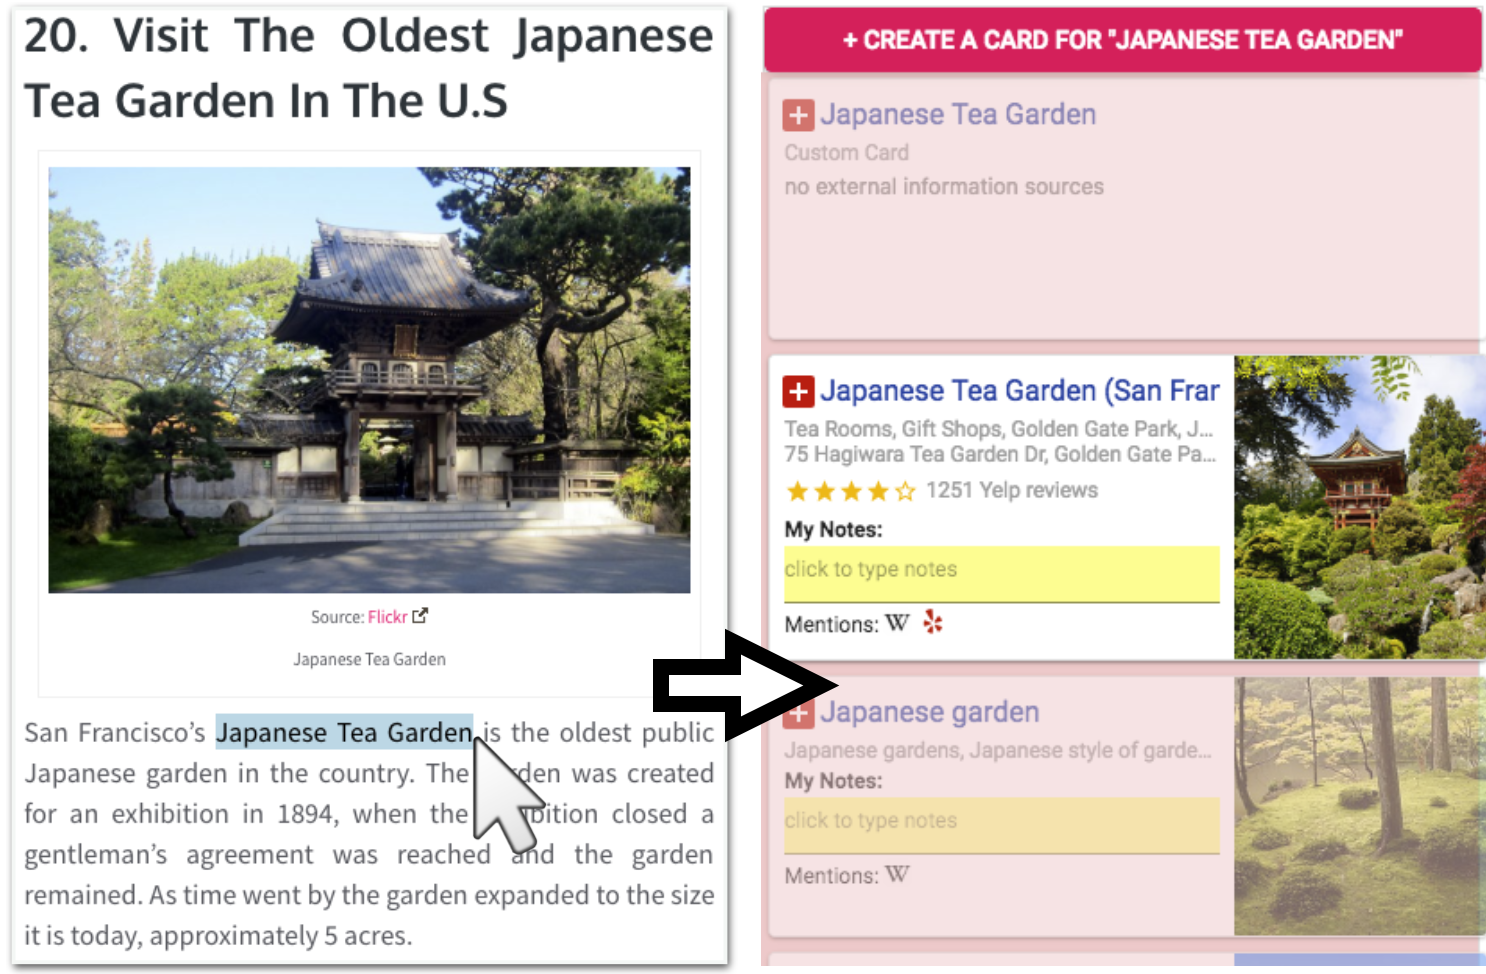
\includegraphics[width=0.6\columnwidth]{Chapters/Fusion/custom4.png}
    \caption{To create a missing entity, users can select a phrase (here, Japanese Tea Garden) on the page and see a list of candidates to choose from. In this case, the top 3 candidates were 1) a Custom Card not linked to external knowledge bases, 2) an Entity Card linked to a specific Japanese garden on both Yelp and DBpedia, and 3) and Entity Card linked to the general entity for Japanese gardens in DBpedia.}
    \label{fig:custom}
\end{figure}


\subsection{Diffusion: Propagating Notes to other Webpages}

After using ``infused'' context to judge the relevance and suitability of options (i.e., entities), users often need to keep track of and organize the options they found valuable. At the same time, users may evaluate newly encountered options against ones they have already saved. Typically this happens by copy-pasting or typing entity names and notes into a separate interface, for example a separate document or email or note taking software (e.g., Evernote). Researchers have tried to lower the switching cost involved in this interaction, for example, by adding a sidebar to the browser for taking free-form notes \cite{notetoself}. However, in the cases when the user encounters additional evidence about an option they already have information about, they need to re-find it in the external system before being able to continue, which can lead to significant adoption issues \cite{notetoself}.

Fusion addresses this challenge this by ``diffusing'' notes that users associate with an entity to all other webpages in the project that also mentioned the same entity, reducing the need for user-driven re-finding. Continuing with our running example of trip planning from the previous subsection, imagine after the user reviewed the information in the restaurant Entity Card, he or she decided to take notes and save the restaurant for future reference. To do so, the user can add various levels of annotation to the card, including just ``hearting'' it to save it in the Saved Cards view as uncategorized  (Figure \ref{fig:main}, top-left corner of E), typing notes about reasons for saving it (Figure \ref{fig:main}, yellow region in E), or selecting sentences (around B) from the webpage to add to the Entity Card as a clip (Figure \ref{fig:main}, E). When the user moved on to other webpages in the project, mentions of the same restaurant will be highlighted in half-height light red (Figure \ref{fig:main}, B), indicating that the user previously interacted with this entity, and upon hovering will see its Entity Card with annotations and clips they have previously added. 

Using this entity-centric approach, users can save notes of information collected across webpages under Entity Cards without having to switch back and forth between the browser and note-taking software, and easily re-find and reuse previously saved information when encountering the same entities on other webpages. To recover from cases where an entity of interest was not recognized by Fusion automatically, users can manually create Entity Cards using interactions as described in the previous subsection. If an user created an Entity Card that was linked to DBpedia and/or Yelp entities, all the information that was associated with them will also appear on the user-created Entity Card. This ensures that users can still save and retrieve information to accumulate what they have learned, even when an entity mention was not automatically recognized by Fusion.

\subsection{Project Overview and Organizing Entities}

\begin{figure*}
    \centering
    \frame{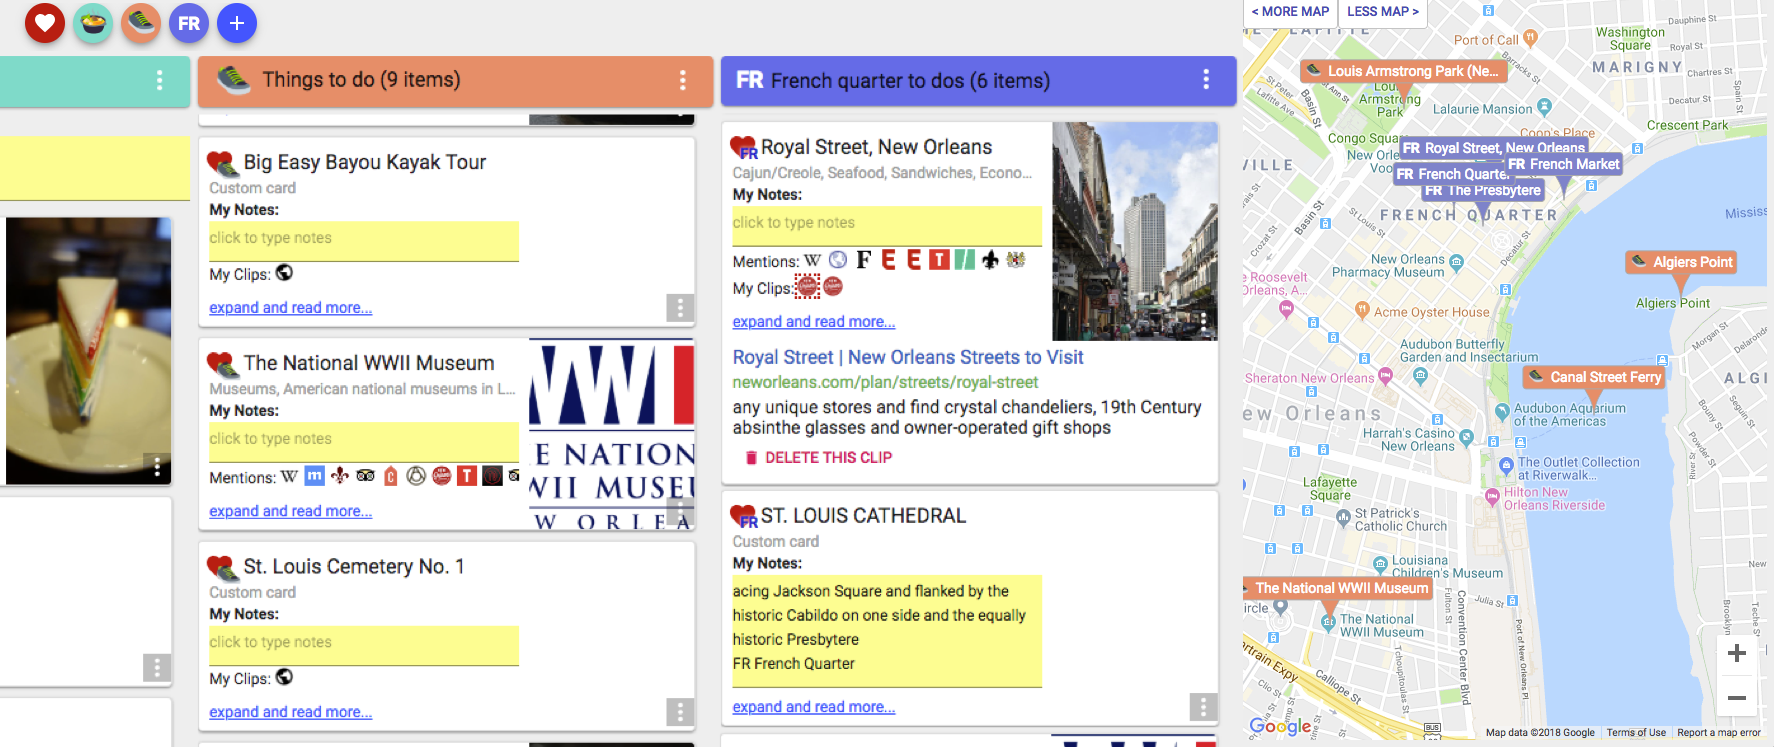
\includegraphics[width=1\textwidth]{Chapters/Fusion/project2.png}}
    \caption{An project overview page created by one participant after searching for 50 minutes, containing entities saved under different categories, text clips from multiple webpages, and typed notes. Custom cards were created, including one for a kayaking tour that was not available on Yelp and DBpedia. The Entity Cards were scaled for clarity in this figure.}
    \label{fig:project}
\end{figure*}


As users in exploratory search tasks gradually progress from discovering entities and gathering evidence to focus more on synthesizing and making decisions, they may also need to organize and compare the collected entities. For example, in a travel planning task, users may want to group their entities into categories of restaurants, attractions, and hotels for comparison, and also to figure out the location and distances between the different entities to plan their trips.

In Fusion, in addition to simply ``hearting'' an Entity Card, users can also create categories with custom names, colors, and icons in the Saved Cards view (Figure \ref{fig:main}, D). To categorize an Entity Card, simply drag and drop it between categories. This allows users to start structuring any time during their exploratory search process when the need arises. Saved geographic entities (entities with coordinates metadata from Yelp and/or DBpedia) will also show up in the Map View  (Figure \ref{fig:main}, C) with their icons and color coded pins. In addition, when users hovered over an unsaved geographic entity on the current webpage, its location is also shown on the Map view. This allows users to better situate a newly encountered option with previously discovered entities to make informed decisions. For example, a user could quickly figure out a hotel recommendation on the current webpage is not relevant by noticing in the Map view that it was too far away from most attractions that they have saved previously on from webpages. At later stages of the exploration process, users might shift their focus from reading and gathering information to synthesizing and organizing information. For this, they can open the Project Overview page by clicking on the expand button in the Saved Cards view to see all their Entity Cards listed in multiple columns of each category along with an integrated map view (Figure \ref{fig:project}).

\subsection{Implementation}

Fusion was built as a addon for the Google Chrome browser. The application uses Google's Firestore real-time database to store mappings between webpages and entities and user-generated data. We utilize the Yelp Search API to fetch entities from Yelp, and uses the open-sourced DBpedia Spotlight \cite{spotlight} software to identify DBpedia entities \cite{dbpedia} in webpages.

\section{Evaluation}
We conducted a lab study to evaluate the benefits of Fusion for users conducting complex exploratory search tasks. The main goal of our study was to explore the benefits and challenges of an entity-centric approach for reading, cross-referencing, and collecting information across multiple webpages in the browser. More specifically, we explored whether participants find our infusion-based, diffusion-based, and organization features to be useful, and whether they consider Fusion as a whole an improvement to their current methods for conducting complex exploratory search tasks. 

\subsection{Lab Study}
We recruited a total of 20 participants (age=19-43, M=25.40, SD=7.67, 55\% female) from a local participant pool. The study began with a pre-survey to collect their demographic information and self-reported expertise in the domain of their assigned condition (described below). Their primary task was to conduct an exploratory search task (50 minutes), and to summarize their findings (5 minutes). Afterwards, participants were given 30 minutes to answer a post-survey about their experiences using Fusion. The study was conducted using 12.5 inch Chromebooks running the latest version of Chrome (v69). Each participant took a total of around 90 minutes to complete the study and was compensated 15 USD. 

The primary domain we aimed to test Fusion on was a travel planning task with the following description:

\begin{quote}
\emph{
You and your friends are going on a trip to New Orleans. Help the group figure out which places you should go and where to eat during the trip. 
}
\end{quote}

\noindent This travel planning task is designed to test Fusion's ability to support collecting and managing evidence from multiple sources for multiple options. Travel planning has a number of characteristics that make it a good task to test new sensemaking and exploratory search approaches, including: information is often scattered across many sources; there is a strong degree of contextualization and personalization needed (e.g., traveling somewhere with kids is very different than without); and evidence such as reviews can be noisy and subjective \cite{zhang2012human,chen2015tripplanner}.  This domain also worked well with the backing knowledge bases in our implementation -- Yelp provided entities for local restaurants and tourist attractions with images and reviews, while DBpedia provided general entities extracted from Wikipedia. We tested Fusion using the travel planning task with 12 randomly selected participants. 


In addition, we also used a camera shopping task with 8 participants using the following description:

\begin{quote}
    \emph{
Your best friend is asking for your help to figure out what DSLR or mirrorless cameras are and which model she should buy. In this task, you will research online to learn what DSLR or mirrorless cameras are, and pick out models that are good for beginners. 
    }
\end{quote}

\noindent The camera shopping task aim to test the boundary conditions of Fusion. Unlike the travel planning task, Fusion's current implementation does not have a knowledge base specialized for camera products, and most webpages in this task do not contain any geographic entities. However, unlike the travel task which assumes only general knowledge, camera shopping for DSLR or mirrorless cameras involves significant learning and necessary expertise with concepts and terms that might be unfamiliar. Participants who were novice in the domain would need to first learn the technical terms and domain knowledge in cameras and photography before advancing to the stage where they can evaluate different options (i.e., camera models) to collect evidence for. In theory, Fusion could also help with general knowledge building using information from DBpedia. For example, helping novice participants to understand and take notes about unfamiliar technical terms (e.g., full-frame CMOS sensors) using Entity Cards from DBpedia. We chose these characteristics to probe the application of an entity-centric approach in a situation where there might not be good coverage of entities and attributes, and where some users might not have the required domain knowledge to evaluate the different options in webpages. 

In both tasks, we also used the following description as a motivator to encourage the participants to put in more research effort, derived from previous studies of sensemaking:

\begin{quote}
    \emph{
Imagine after this task you will share your project overview page with your friend(s), along with a short summarization in an email. To convince your friend(s) of your choices, provide enough reasons and information about your choices.
    }
\end{quote}

\noindent After participants finished the primary task, they were given 30 minutes to answer a post-survey about their experiences with Fusion and to compare Fusion with their current practice.

\subsection{Results}

\begin{table}
  \centering
  \scriptsize

% question, number of sources, number of clips, number of turkers
  \begin{tabular}{ r  r l |  r l |  r l }
    \hline
	&
	\multicolumn{2}{c}{} &
	\multicolumn{2}{c}{Camera} &
	\multicolumn{2}{c}{Camera} \\
	
	\multicolumn{1}{c}{Statement} &
	\multicolumn{2}{c}{Travel} &
	\multicolumn{2}{c}{(experts)} &
	\multicolumn{2}{c}{(novices)} \\
	
    
	\hline
	
	\multicolumn{1}{p{0.54\columnwidth}}{P1.\textit{Pre-survey: I understand what DSLR cameras are}} &
	\multicolumn{2}{c|}{-} &
    6.75 & $\sigma$=0.50 &
    3.50 & $\sigma$=1.73 \\
    
	\hline
	
    
	\multicolumn{1}{p{0.54\columnwidth}}{Q1.\textit{Fusion is an improvement to my current practice}} &
    5.67  & $\sigma$=1.11 &
    5.75 & $\sigma$=0.50 &
    2.75 & $\sigma$=2.22 \\
    
	\multicolumn{1}{p{0.54\columnwidth}}{I1.\textit{The cards were useful for reading \& learning new things}} &
    5.42 & $\sigma$=1.11 &
    6.00 & $\sigma$=0.82 &
    3.25 & $\sigma$=2.63 \\
    
	\multicolumn{1}{p{0.54\columnwidth}}{I2.\textit{Information from Yelp was useful
}} &
    5.92 & $\sigma$=0.86 &
	\multicolumn{2}{c|}{-} &
	\multicolumn{2}{c}{-} \\
    
	\multicolumn{1}{p{0.54\columnwidth}}{I3.\textit{Information from Wikipedia was useful}} &
    5.67 & $\sigma$=0.85 &
    5.50 & $\sigma$=1.29 &
    4.00 & $\sigma$=2.45 \\
    
	\multicolumn{1}{p{0.54\columnwidth}}{I4.\textit{Information from other webpages was useful}} &
    5.58 & $\sigma$=1.11 &
    4.75 & $\sigma$=0.96 &
    4.50 & $\sigma$=2.08 \\
    
    
	\multicolumn{1}{p{0.54\columnwidth}}{D1.\textit{Cards allowed me to quickly refer to things saved across pages}} &
    6.00 & $\sigma$=0.71 &
    5.25 & $\sigma$=1.70 &
    4.00 & $\sigma$=2.45 \\
    
	\multicolumn{1}{p{0.54\columnwidth}}{D2.\textit{Cards were useful because I don't have to switch to other programs to save notes}
} &
    6.33 & $\sigma$=0.85 &
    6.00 & $\sigma$=0.82 &
    4.25 & $\sigma$=2.06 \\
    
	\hline
	
	
	&
	\multicolumn{2}{r}{N=12} &
	\multicolumn{2}{r}{N=4} &
	\multicolumn{2}{r}{N=4} \\
	
  \end{tabular}
  \caption{Mean statistics for Likert-scale responses from the lab study. A score of 1 indicates strong disagreement with the statement and 7 indicates strong agreement. Participants under the DSLR Camera shopping task were split into two groups based on their self-reported domain expertize in the pre-survey.}
  \label{tab:fusion_results}
\end{table}

Table \ref{tab:fusion_results} shows the mean statistics for Likert-scale responses on questions regarding different specific features of Fusion, with a score of 1 indicating strongly disagreement with the statement and a score of 7 indicating strong agreement. In terms of prior knowledge, none of the 12 participants in the travel task reported having ever traveled to New Orleans, and conduct travel planning once to a few times per year (11) or once in a few years (1). However, we discovered that the DSLR camera task had very different characteristics for the 4 participants who either strongly agreed or agreed that they understand what DSLR cameras are (N=4, M=6.75, SD=0.5) versus the 4 camera novices who did not (N=4, M=3.50, SD=1.73). While the domain experts used Fusion for collecting information about various cameras, the novices largely spent their time reading webpages to understand the various terminologies and differences between camera types. Thus in the analyses below we report on these two groups separately.

Overall, participants in the travel planning task (N=12) and expert participants in the camera shopping task (N=4) considered Fusion to be an improvement when compared to their current practices (Q1, M=5.67, 5.75), and found both infusion-based (D1, M=6.00, 5.25) and diffusion-based features (I1, M=5.42, 6.00) to be useful. On the other hand, novice participants in the camera shopping task saw less value in the system (M=2.75, SD=2.22. See Table \ref{tab:fusion_results}). Instead of actively collecting evidence and saving different entities (i.e., camera models), novice participants typically spent time reading and learning about general knowledge topics for DSLR cameras and photography. While we originally expected Fusion to be beneficial for general knowledge building by allowing users to quickly look up the definition of unfamiliar terminologies and concepts using the entity descriptions from DBpedia, participants did not find the short description from DBpedia beneficial for this purpose (M=4.00, SD=2.45).  This suggests that Fusion might be of more benefit to the gathering and deciding stages of sensemaking than early learning, although it is possible that with more appropriate descriptions or additional information an entity-centric approach might still be beneficial. Given that novices largely spending their time reading and did not have an opportunity to interact significantly with Fusion's features, below we focus on the results from the travel task and the camera experts.


\subsubsection{\textbf{Infusion-based Features}}

Travel and expert camera participants found the Infusion-based features to be useful for evaluating new options (I1, M=5.42,6.00; SD=1.11,0.82; N=12,4). In addition to the using entity evidence gathered by Fusion, they also described how the lightweight interaction relieved them from the need to create additional searches:

\begin{quote}
``[The Entity Cards were useful because] I liked seeing similar material and being able to continue research without having to do an actual search''
\end{quote}

\noindent At the same time, it also helped them discover and navigate useful alternative information sources, which was not our original design intention:

\begin{quote}
``[The Entity Cards were useful because] i was taken to mentions on sites i would not have thought of''
\end{quote}

\begin{quote}
``[The Entity Cards were useful because they] Gives you info about other websites that might be useful later on.''
\end{quote}

\begin{quote}
``[The Entity Cards were useful because] if i found a restaurant and saw it was also mentioned on yelp i could go read reviews and find similar, interesting restaurants''
\end{quote}

\noindent Participants also described using infusion-based features as a way to verify uncertain information on the current webpage:

\begin{quote}
``[The mentions from other webpages were useful because they] allowed me to see if the comments on this page was true.''
\end{quote}

\begin{quote}
``[The mentions from other webpages were useful because] I can know its exact condition other than the advertisements provided by the own company.''
\end{quote}

\noindent Conversely, other participants in the camera shopping task described how they would prefer to use information sources that were familiar and trusted to them instead of webpages returned from search engines:

\begin{quote}
``[The mentions from other webpages were not useful because] mkbhd [Marques Brownlee] and others are good tech reviewers and they can provide a better pro vs con list than reading [the mentions]..''
\end{quote}

\noindent This suggest a future direction for personalizing the Entity Cards to prioritize using sources trusted by users.

\subsubsection{\textbf{Diffusion-based Features}}

Participants found the diffusion-based features to be useful for accessing previously saved information without keeping multiple tabs opened, as well as for accumulating knowledge across webpages about different options in order to make decisions: 

\begin{quote}
``[Being able to save notes on the Entity Cards was useful because] I could compound things that i had already said and supplement my knowledge to helping me arrive at a decision''
\end{quote}

\begin{quote}
``They [the Entity Cards] were very useful when i needed to pull up information on something I tagged, without the need to use multiple tabs...'' 
\end{quote}

\noindent On the other hand, they also described how saving notes under Fusion required less effort when compared to using external word processors:

\begin{quote}
``i liked that i could save entities with notes attached and look back at them all put together. i used to do this with a word doc and links and it wasn't nearly as easy''
\end{quote}

\noindent This shows our diffusion-based features that actively resurface saved information not only allowed useful notes to be reused, but also allowed users to build on previously knowledge and progress towards informed decisions. Interestingly, participants also described how having entity cards to organize their clips and notes lowered the cost of removing information that was no longer useful from their workspace:

\begin{quote}
``They [the Entity Cards] were very useful... i could save anything, and if i didn't need it later it was simple to erase''
\end{quote}

\noindent Both the reusing of previously saved notes and the removing of notes that were no longer relevant were issues identified in previous work that allowed participants to save notes persisted across webpages \cite{notetoself}. Our findings suggest the entity-centric approach of Fusion can potentially address these issues, allowing participants to collect evidence and accumulate knowledge while at the same time maintain a manageable workspace with less irrelevant information. 

\section*{Limitations}

Participants also pointed to issues they encountered during the study, which inform ways to improve future versions of Fusion so it can be adopted by a wide range of domains and scenarios.
One common theme was the high effort of capturing missing structured entity attributes from the webpages. Participants in the travel planning task further pointed to the lack of support to save structured attributes, such as a missing address and the corresponding inability to pin an entity on the Map view. 

\begin{quote}
``Easy to make a record, but not easy to record all the information I need, such as address, and photos.``
\end{quote}

\begin{quote}
``[Improve Infuse by allowing me to] Mark the address on google map if a place doesn't have an existing map location.'' 
\end{quote}

\noindent Similarly, participants in the camera shopping task cited the high cost of capturing camera specifications:

\begin{quote}
``The cards did not provide any additional information about the cameras. However, they were useful in keeping track of the features of different cameras.''
\end{quote}

\noindent While DBpedia actually contain detailed specification of many DSLR camera models,\footnote{http://dbpedia.org/page/Canon\_EOS\_750D} entities in DBpedia typically have dozens to hundreds of attributes. Fusion only surfaced the most common attributes (i.e., location, short description, and categories) so it does not overwhelm users. Future work could involve better extracting structured information, for example looking at alignment between DBpedia information and information on the page, or structured information extraction from webpages through end-user interaction \cite{thresher,bier2006entity}.
Finally, while participants did not make many comments about the simple category structure provided by Fusion for managing Entity Cards, they did point to the need for further synthesizing the collected information. This includes writing out a travel itinerary using a word processor or calendar software, and also accessing collected information on mobile platforms:

\begin{quote}
``Fusion is helpful in the first stage of information collection, but when it comes to the final detailed plan of the trip, I still need more place for editing, adding specific time and so on. Also I need to access my plan through my phone, so the calendar or memo are more useful during the trip.''
\end{quote}


\section{Discussion and Future Work}


Results suggest participants found Fusion to be an improvement to their current practice, and valued both infusion- and diffusion-based features. However, we also learned that adoption may be critically sensitive to the cost structure of extracting entities and attributes. Some limitations identified by our participants can potentially be addressed with approaches in previous work. For example, using end-user interactions to bootstrap entity-attribute extractors \cite{thresher,bier2006entity}.

We think the entity-centric approach can support exploratory tasks in a wide variety of domains involving identifying potential options and collecting evidence. However, the cost of adapting the current framework to support different domain is unclear, especially for domains where high quality knowledge bases are not readily available. In the post-survey, we also asked participants if they could think of other search tasks that may benefit from using Fusion, and participants pointed to a variety of different tasks, including essay writing, event planning, literature review, job searching, and deciding on a college major. 

Many other future research directions present themselves. For example, automatically summarizing evidence gathered across different websites for an entity instead of simply listing them could help Fusion scale to much larger projects with many sources, while keeping gathered information easy to consume for the users. However, how to surface information sources in the summarization so users can better evaluate the trustworthiness of the pieces of information is still an open problem. While Fusion supported synthesizing entities and evidence into categories, providing support for creating different structures (e.g., tables or essays) still needs further investigation.

Our results have implications for the design of future intelligent browser interfaces that can better understand the information being consumed by its users, and building novel interactive systems for supporting online sensemaking. As phenomena such as fake news and shill reviews have demonstrated, there are significant drawbacks to the easy availability and generation of online content. Interactive systems that can provide additional context to users in situ may become increasingly necessary to help navigate the information overload. Anecdotal evidence for this need can also been seen in the rise of aggregation-based sites such as Metacritic or Wirecutter, which act as virtual meta-analyses of evidence and opinions but fail to take into account the personal context of the user and their goals. We believe that this work presents a step forward in illustrating a design space for interactive systems which can take advantage of advances in machine learning and natural language processing to help end users actively gain context and personalize their online sensemaking activities.


%\section{Conclusion} %(or remove the below)
%We introduced Fusion, a browser addon that enable the browser to better understand information consumed by its users for supporting sensemaking across webpages while conducting complex exploratory search tasks. Traditional approaches for supporting exploratory search tasks either try to generate better search results page or with an external interface for organizing saved information. We instead use an entity-centric approach to support the process of collecting and organizing evidence from multiple information sources. Fusion empowers users to better evaluate entities with relevant information ``infused'' from other webpages, and allows users to ``diffuse'' their notes about an entity across different webpages where the same entity was mentioned. In our user study about trip planning, participants valued both infusion-based and diffusion-based features, and considered Fusion an improvement to their current practices.

